\lhead[\thepage]{CAPÍTULO \thechapter. IMPLEMENTACIÓN Y DESPLIEGUE}
\chead[]{}
\rhead[WepSIM: Simulador de un procesador elemental con unidad de control microprogramada\leftmark]{\thepage}
\renewcommand{\headrulewidth}{0.5pt}

\lfoot[]{}
\cfoot[]{}
\rfoot[]{}
\renewcommand{\footrulewidth}{0pt}

%% This is an example first chapter.  You should put chapter/appendix that you
%% write into a separate file, and add a line \include{yourfilename} to
%% main.tex, where `yourfilename.tex' is the name of the chapter/appendix file.
%% You can process specific files by typing their names in at the 
%% \files=
%% prompt when you run the file main.tex through LaTeX.
\chapter{Implementación y despliegue}
\label{ch:implementation_and_deployment}
\markboth{}{IMPLEMENTATION}


Este capítulo trata la implementación y despliegue del software. En cuanto a la implementación del sistema, se explican las partes más complicadas del código en (Sección  \ref{sec:implementation}, \textit{\nameref{sec:implementation}}). Por otro lado, explicamos los pasos necesarios para desplegar el sistema final (Sección \ref{sec:deployment}, \textit{\nameref{sec:deployment}})


\section{Implementación}
\label{sec:implementation}


Como hemos explicado en el Capítulo \ref{ch:analysis}, \textit{\nameref{ch:analysis}}, hemos implementado el simulador utilizando el lenguaje de programación JavaScript junto con HTML, CSS y las bibliotecas/frameworks JQuery, JQueryUI, JQuery Mobile, Knockout y BootStrap. El motor de simulación es el encargado de ejecutar cada uno de los ciclos de reloj del simulador, tomando como entradas tanto el modelo hardware como el modelo software, pero el desarrollador ha debido de diseñar e implementar el algoritmo que posibilita esta ejecución.

Además, hemos trabajado en conseguir una herramienta que sea capaz de generar la memoria de control mediante la definición del juego de instrucciones por parte del usuario, y de generar el código binario asociado al código ensamblador definido por el usuario; el cual depende del juego de instrucciones definido previamente. Para ello, se han diseñado e implementado dos compiladores diferentes, capaces de generar los binarios correspondientes además de las estructuras de datos necesarias para ayudar al motor de simulación a lo largo de la ejecución.

\begin{figure}[htbp]
 	\centering
 	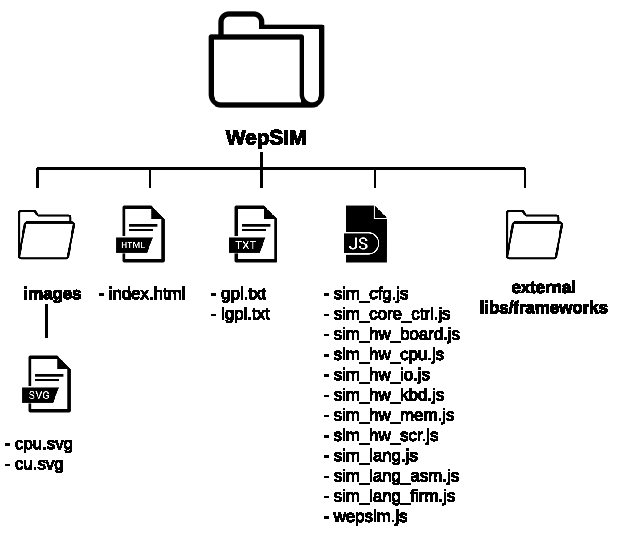
\includegraphics[width=10cm]{figures/folder_diagram}
 	\caption{Estructura de ficheros.}
	\label{fig:folder_structure}
\end{figure}

Como resultado de este diseño e implementación, el código fuente de la herramienta está compuesto por una serie de ficheros que definen las funcionalidades y componentes anteriormente citados. Por ello, es necesario explicar la estructura de ficheros que componen el simulador y las dependencias que existen entre sí. De esta forma, en la Figura \ref{fig:folder_structure} podemos ver los ficheros que componen la herramienta web, los cuales tienen una serie de dependencias indicadas en la Figura \ref{fig:files_dependencies}.

\begin{figure}[htbp]
 	\centering
 	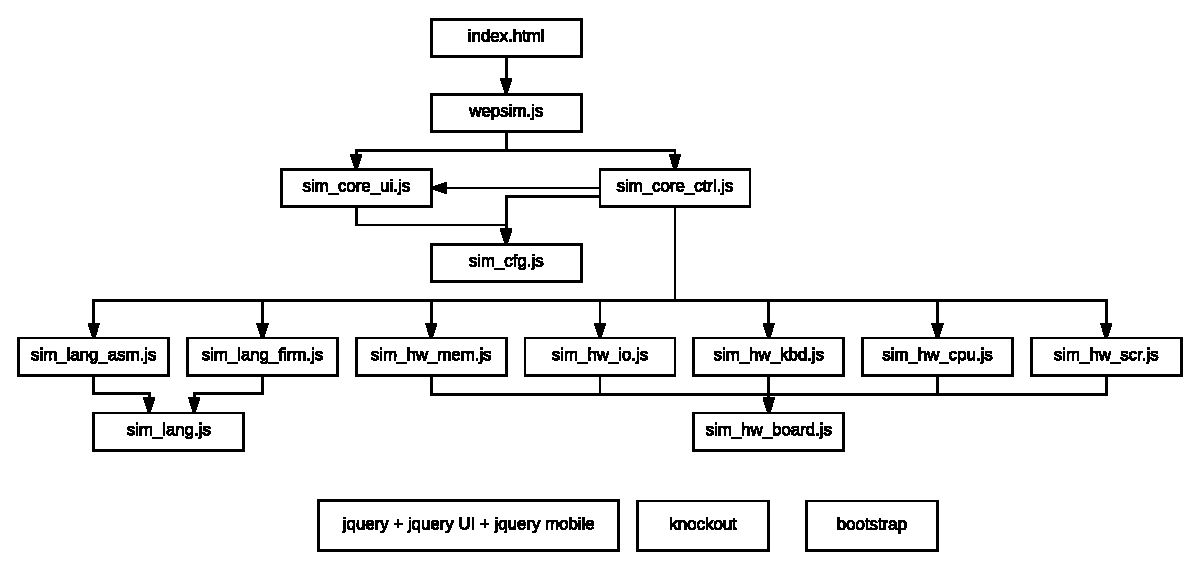
\includegraphics[width=15.5cm]{figures/dependencies_diagram}
 	\caption{Dependencias entre ficheros.}
	\label{fig:files_dependencies}
\end{figure}

Los ficheros que componen WepSIM son detallados a continuación:

\begin{itemize}

\item \textbf{index.html: } este fichero se encarga de la vista de la herramienta, generando la interfaz de usuario de la herramienta.

\item \textbf{gpl.txt y lgpl.txt: } estos ficheros contienen la especificación de las licencias del software.

\item \textbf{sim\char`_cfg.js} este fichero contiene las estructuras de datos de la configuración de la herramienta.

\item \textbf{sim\char`_core\char`_ctrl.js:}  este fichero contiene la implementación del motor de simulación de la herramienta.

\item \textbf{sim\char`_core\char`_ui.js: } este fichero contiene la implementación del motor de la interfaz de usuario de la herramienta.

\item \textbf{sim\char`_hw\char`_cpu.js: } este fichero contiene la definición del modelo hardware de la cpu del simulador.

\item \textbf{sim\char`_hw\char`_io.js: } este fichero contiene la definición del modelo hardware del módulo de generación de interrupciones del simulador.

\item \textbf{sim\char`_hw\char`_kbd.js: } este fichero contiene la definición del modelo hardware del módulo del teclado del simulador.

\item \textbf{sim\char`_hw\char`_scr.js: } este fichero contiene la definición del modelo hardware de la memoria principal del simulador.

\item \textbf{sim\char`_hw\char`_mem.js: } este fichero contiene la definición del modelo hardware de la pantalla del simulador.

\item \textbf{sim\char`_lang.js: } este fichero contiene la implementación de las funciones principales del parser de ficheros de la herramienta.

\item \textbf{sim\char`_lang\char`_asm.js: } este fichero contiene la implementación del compilador de código ensamblador de la herramienta.

\item \textbf{sim\char`_lang\char`_firm.js: } este fichero contiene la implementación del compilador de microcódigo de la herramienta.

\item \textbf{images/cpu.svg: } este fichero contiene la definición de la imagen vectorial de la cpu de la herramienta.

\item \textbf{images/cpu.svg: } este fichero contiene la definición de la imagen vectorial de la unidad de control de la herramienta.

\item \textbf{external folder: } este directorio contiene las bibliotecas y frameworks que necesita el simulador para su correcto funcionamiento, como son JQuery, JQueryUI, JQuery Mobile, Knockout y BootStrap.

\end{itemize}

Para comprender funcionamiento tanto de los dos compiladores utilizados (compilador de microcódigo y compilador de ensamblador) como del kernel del simulador, se puede observar en el Pseudocódigo \ref{alg:firmware_compiler_pseudocode}, mientras que en el Pseudocódigo \ref{alg:assembly_compiler_pseudocode} podemos ver el proceso de compilación del código ensamblador definido por el usuario en función de la memoria de control previamente generada, detallando el proceso de compilación del segmento de datos en el Pseudocódigo \ref{alg:data_segment_pseudocode} y el proceso de compilación del segmento de texto en el Pseudocódigo \ref{alg:text_segment_pseudocode}. En el Pseudocódigo \ref{alg:core_simulator_pseudocode} podemos ver como se realiza una simulación, realizando la comprobación de segmentos de memoria, tipo de simulación, y ejecución del ciclo o instrucción correspondiente.

El proceso de compilación del juego de instrucciones (Pseudocódigo \ref{alg:firmware_compiler_pseudocode}) se realiza mediante un análsis sintáctico basado en la técnica \textit{\gls{lexyacc}}, que queda perfectamente descrita en \cite{bennett1996introduction}. De este modo, el proceso de compilación queda dividido en tres bloques importantes: instrucciones, nombrado de registros y pseudoinstrucciones. En primer lugar, se realiza la lectura del bloque de instrucciones, en donde se comprueba cada uno de los campos y parámetros que la conforman para posteriormente generar el binario asociado a cada ciclo de reloj. Después, se realiza la lectura del banco de registros, donde se forma el par \textit{id,nombre}, pudiendo realizar el nombrado deseado de los distintos registros que lo componen. Por último, se realiza la lectura de pseudoinstrucciones. Estas instrucciones no pertenecen al lenguaje, sino que están compuestas por instrucciones del lenguaje, pudiendo el usuario utilizar técnicas de alto nivel en donde con una única línea de código, genere más de una instrucción.

\clearpage

\begin{algorithm}[h]
	\caption{Proceso de compilación del juego de instrucciones.}
	\label{alg:firmware_compiler_pseudocode}
  	\scriptsize
  	\setstretch{1.35}
	\begin{algorithmic}[1]
		\Function{compile\_firmware}{$context$ }
		\State $token$ = getToken();
		\State $firmware$ = $null$;
		\State $instructions $= $null$;
		\State $registers$ = $null$;
		\State $pseudoinstructions$ = $null$;
		\While {(!is\_registers($token$) and $token$ != $null$)}
			\State $instruction = null$;
			\State $instructions$[$signature$]=readSignature(getNextToken());
			\State $instructions$[$co$]=readCo(getNextToken());
			\If{(getNextToken() == $COP$)}
				\State $instruction$[$cop$]=readCop(getNextToken());
			\EndIf
			\While {(is\_Field(getNextToken())}
				\State $instructions$[$field$].add=readField(getToken());
			\EndWhile
			\While {(is\_microcode(getNextToken())}
				\State $instructions$[$microcode$].add=readCycle(getToken());
			\EndWhile
			\State $firmware$.add($instructions$);
		\EndWhile
		\If{(is\_registers(getToken())}
			\State $registers$ = readRegisters(getToken());
		\EndIf
		\If{(is\_pseudoInstructions(getToken())}
			\State $pseudoinstructions$ = readPseudoinstructions(getToken());
		\EndIf
		\State $firmware$.add($instructions$);
		\State $firmware$.add($registers$);
		\State $firmware$.add($pseudoinstructions$);
		\State Return $firmware$;
		\EndFunction
	\end{algorithmic}
\end{algorithm}

\clearpage

El proceso de compilación del código ensamblador (Figura \ref{alg:firmware_compiler_pseudocode}) está basado, al igual que el compilador del juego de instrucciones, en la técnica de compilación \textit{\gls{lexyacc}}. Este proceso, está dividido en dos etapas: segmentos de datos y segmento de texto.

En la etapa de compilación del segmento de datos, se realiza el proceso de lectura y compilación de las diferentes directivas definidas por el usuario. En primer lugar, se realiza la identificación de las diferentes etiquetas que identifican a las directivas y que serán utilizadas posteriormente en el segmento de texto. Una vez identificadas estas etiquetas, se procede a la generación del binario asociado a este segmento, el cual depende directamente del tipo de directiva utilizado y del tamaño de la directiva.

\begin{algorithm}[h]
	\caption{Proceso de compilación de código ensamblador.}
	\label{alg:assembly_compiler_pseudocode}
  	\scriptsize
  	\setstretch{1.35}
	\begin{algorithmic}[1]
		\Function{compile\_assembly}{ $context$,$datosCU$}
		\State $dataSegment$ = $null$;
		\State $textSegment$ = $null$;
		\State $mainMemory$ = $null$;
		\If{(!is\_data\_segment(getToken()))}
			\State Return;
		\EndIf
		\State $dataSegment$ = read\_data\_segment($context$[$dSegment$]);
		\If{(!is\_text\_segment(getToken()))}
			\State Return;
		\EndIf
		\State $textSegment$ = read\_text\_segment($context$[$tSegment$]);
		\State $mainMemory$.add($dataSegment$);
		\State $mainMemory$.add($textSegment$,$dataSegment$.$labels$);
		\State Return $mainMemory$;
		\EndFunction
\end{algorithmic}
\end{algorithm}

En la etapa de compilación del segmento de texto, se realiza el proceso de compilación de las diferentes instrucciones ensamblador definidas por el usuario. Por ello, es necesario el uso del juego de instrucciones definido previamente, ya que la generación del binario de la instrucción depende de la definición previa. En primer lugar, se realiza la búsqueda de las diferentes etiquetas empleadas en este segmento, identificando las nuevas etiquetas definidas a las anteriores definidas en el segmento de datos, para la cambiar la etiqueta por el valor de la dirección de memoria asociada a la etiqueta. Una vez realizado este proceso, se procede a la compilación de cada una de las instrucciones, buscando para cada instrucción del segmento de texto una instrucción definida en el juego de instrucciones que cumple con la sintaxis. En caso de existir la instrucción, se procede a la generación del binario asociado, comprobando el valor de cada uno de los campos. Este proceso se realiza para cada una de las operaciones definidas en este segmento. Una vez traducidas todas las instrucciones, se genera la memoria principal asociada al código definido.

Por último, se indica el proceso de simulación de la herramienta. Este proceso es realizado en el kernel del simulador como ha sido explicado anteriormente (Sección \ref{sec:kernel_simulator}). Como podemos observar en el Pseudocódigo \ref{alg:core_simulator_pseudocode}, en primer lugar se realiza la petición de ejecución. El controlador del simulador, comprobaría el contexto (\textit{breakpoints}, final de segmento, etc.) verificando si la ejecución es posible. En caso de ser posible, identificaría el tipo de simulación solicitada, llamando a la función correspondiente. Si la ejecución solicitada es de una microinstrucción, el motor de simulación únicamente generaría un ciclo de reloj, enviándolo al modelo hardware para su ejecución y actualizando posteriormente los valores mostrados en la interfaz de usuario. La ejecución de una instrucción completa se realiza ejecutando en bucle la secuencia de microinstrucciones correspondientes hasta que el registro de microdirección apunta a la dirección de comienzo del ciclo \textit{FETCH}, que indicaría el comienzo de la próxima instrucción, o apunta a una dirección de memoria fuera del rango del segmento de texto, lo cual indica que la simulación del código ensamblador ha finalizado.

En \cite{wepsimManualUser} se presenta el manual completo de usuario de la herramienta, que incluye la especificación del modelo hardware implementado y la explicación de uso del simulador, indicando algunos ejemplos docentes para aprender el uso de esta herramienta y poder comprender mejor el funcionamiento de los distintos componentes que la forman.

\begin{algorithm}[h]
	\caption{Proceso de compilación de código ensamblador: segmento de datos.}
	\label{alg:data_segment_pseudocode}
  	\scriptsize
  	\setstretch{1.35}
	\begin{algorithmic}[1]
		\Function{read\_data\_segment}{$context$}
			\State $labels$ = $null$;		
			\State $token$ = getToken();
			\While {(!is\_End(getNextToken())}   \Comment{Check Labels}
				\If{(isLabel(getToken()))}
					\State $labels$.add(getLabel(getToken()));
				\EndIf
			\EndWhile
			\State $dataSegment$[$labels$].add(labels);
			\State $token$ = getFirstToken();
			\For{($i$ in $context$[$directives$])}	\Comment{Read Directives}  
				\State $possible\_datatype$ = $i$;
				\If{($possible\_datatype$ == "$.byte$")}
					$dataSegment$[$directives$].add(readByte($i$));
				\EndIf
				\If{($possible\_datatype$ == "$.half$")}
					$dataSegment$[$directives$].add(readHalf($i$));
				\EndIf
				\If{($possible\_datatype$ == "$.word$")}
					$dataSegment$[$directives$].add(readWord($i$));
				\EndIf
				\If{($possible\_datatype$ == "$.space$")}
					$dataSegment$[$directives$].add(readSpace($i$));
				\EndIf
				\If{($possible\_datatype$ == "$.ascii$")}
					$dataSegment$[$directives$].add(readAscii($i$));
				\EndIf
				\If{($possible\_datatype$ == "$.asciiz$")}
					$dataSegment$[$directives$].add($i$));
				\EndIf
				\If{($possible\_datatype$ == "$.align$")}
					$dataSegment$[$directives$].add(readAlign($i$));
				\EndIf
			\EndFor
			 \State Return $dataSegment$
		\EndFunction
	\end{algorithmic}
\end{algorithm}

\begin{algorithm}[h]
	\caption{Proceso de compilación de código ensamblador: segmento de texto.}
	\label{alg:text_segment_pseudocode}
  	\scriptsize
  	\setstretch{1.35}
	\begin{algorithmic}[1]
		\Function{read\_text\_segment}{$context$,$labels$}
			\For {($i$ in $labels$}    \Comment{Read Labels}
				\State replaceLabel($context$, $i$);	   \Comment{Replace Label in Text Segment}
			\EndFor
			\For{($i$ in $context$[$instructions$])}     \Comment{Read Instructions}
				\State $auxInstruction$ = fillFields($i$);
				\State $auxBinary$ = $null$;
				\If{(!isInstruction($auxInstruction$[$0$]))}     \Comment{Check if instruction exist}
					\State Return;
				\EndIf
				$auxBinary$ = generateBinary($auxInstruction$);
				\If{($auxBinary$ == $null$)}
					\State Return;
				\EndIf
				$textSegment$.add($auxBinary$);
			\EndFor
			 \State Return $textSegment$
		\EndFunction
	\end{algorithmic}
\end{algorithm}


\begin{algorithm}[h]
	\caption{Proceso de simulación.}
	\label{alg:core_simulator_pseudocode}
  	\scriptsize
  	\setstretch{1.35}
	\begin{algorithmic}[1]
		\Function{run\_simulation}{ }
		  \If {(!possible\_execute())}
		    \State Return;
		  \EndIf		
		  \State change\_play\_button();
		  \State execute\_simulation\_inchain();
		\EndFunction
		\Function{execute\_simulation\_inchain}{ }
		   \If {(end\_code())}
		    \State Return;
		   \EndIf	
		   \If {(is\_breakpoint())}
		    \State Return;
		   \EndIf	
		   \If{(execute\_mode == microInstruction)}
		         \State{execute\_microInstruction();}
		   \EndIf
		   \If{(execute\_mode == instruction)}
		         \State{execute\_instruction();}
		   \EndIf	
		\EndFunction
		\Function{execute\_microInstruction}{ }
		\If {(!possible\_execute())}
		    \State Return;
		\EndIf
		\State compute\_general\_behaviour(CLOCK); \Comment{Execute Cycle}
		\State update\_UI();		
		\EndFunction
		\Function{execute\_instruction}{ }
		\If {(!possible\_execute())}
		    \State Return;
		\EndIf
		\Do
		\State compute\_general\_behaviour(CLOCK); \Comment{Execute Cycle}
		\doWhile{($reg\_microaddr$!=$0$ and $mem\_control$[$microAddr$]!=$undefined$)} \Comment{Check Next Cycle}
		\State update\_UI(); \Comment{Update User Interface}
		\EndFunction
	\end{algorithmic}
\end{algorithm}
\clearpage

\section{Despliegue}
\label{sec:deployment}

En esta sección se presenta el despliegue de la herramienta, el cual queda dividido en tres partes: especificaciones técnicas recomendadas, el proceso de despliegue del software para que sea accesible, y por último el proceso de ejecución de la herramienta.

Las especificaciones técnicas recomendadas para que el usuario final obtenga la mejor experiencia posible con la herramienta son:

\begin{itemize}

\item \textbf{Sistema Operativo}: Ubuntu 16.04.2 LTS (\emph{Linux distribution}) /Windows 10 / MacOS 10.12.5.

\item \textbf{Procesador}: Intel(R) Core(TM) i3 CPU 6300 @3.8GHz o superior.

\item \textbf{\gls{ram}}: 2 GB o superior.

\item \textbf{Almacenamiento}: 1 GB de espacio libre en el disco duro (recomendado para el navegador web).

\item \textbf{Red}: La conexión a internet no es necesaria para la ejecución de la herramienta, únicamente para el acceso a ella.

\item \textbf{Software}: Los siguientes navegadores web son los recomendados para el uso de la herramienta:

	\begin{itemize}

	\item[1.] Mozilla Firefox 45+.
	
	\item[2.] Google Chrome 50+.
	
	\item[3.] Microsoft Edge 30+.
	
	\item[4.] Safari 10+.

	\end{itemize}

\end{itemize}

Para el proceso de despliegue de la herramienta, se requiere que el usuario disponga de un servidor web \textit{Apache}  o \textit{Nginx} instalado en su computador para que el software sea accesible. Una vez instalado el servidor web, se deben de seguir los siguientes pasos:

\begin{itemize}

	\item[1.] Acceder al directorio establecido en el servidor web para alojar el simulador.

	\item[2.] Clonar el repositorio del simulador para obtener el código fuente del simulador:
	
	 \textbf{\textit{git clone https://github.com/wepsim/wepsim.git}}
	
	\item[3.] Reiniciar el servicio del servidor web para que realice los cambios pertinentes.

\end{itemize}

Por último, el usuario podrá acceder a la herramienta mediante un navegador web de los citados anteriormente. Para ello, el usuario deberá de indicar en el navegador la dirección en la cual ha sido publicada la herramienta, no siendo necesaria la conexión a Internet en caso de estar publicada en el mismo computador (\textit{localhost}).

En caso de no desear el usuario realizar este proceso, puede acceder a la herramienta de forma inmediata accediendo a la dirección: 

\url{https://wepsim.github.io/wepsim/}.